

\subsubsection{BLE基地局情報を用いた初期進行方向の補正}

フロアマップ情報を用いた初期進行方向補正ではマップの
存在可能な点の分布によっては正しく機能しない場合があり,
別の方法としてBLEビーコンの基地局の位置情報を用いた
初期進行方向補正を行う関数をListing\ref{lst:rotate-trajectory-using-ble}に示す.
この関数では加速度DF,角度DF,BLEビーコンの受信電波DF, BLEビーコンの基地局DFを受け取る.
BLEビーコンの受信電波DFとBLEビーコンの基地局DFのカラム名とデータ型を表6,表7に示す.
戻り値は角度DFと座標DFを返す.
フロアマップ上に存在する全てのBLEビーコンの基地局の位置情報を図\ref{fig:ble-beacon-position}に示す.
一定の強いRSSIの電波を受信した際の時間情報を基に時間的に近い推定軌跡の座標を取得する.
図\ref{fig:ble-merge}に示した図は時間的に近い推定軌跡の座標を時間経過に応じた色で表しており
青色の座標が配置されたBLEビーコンの座標を表している.
推定した軌跡の受信したBLEビーコンの基地局の座標との距離を計算する.
この総和が最小となるような回転角度をグリッドサーチで探し最適な角度に補正を行う.

\begin{figure}[ht]
	\centering
	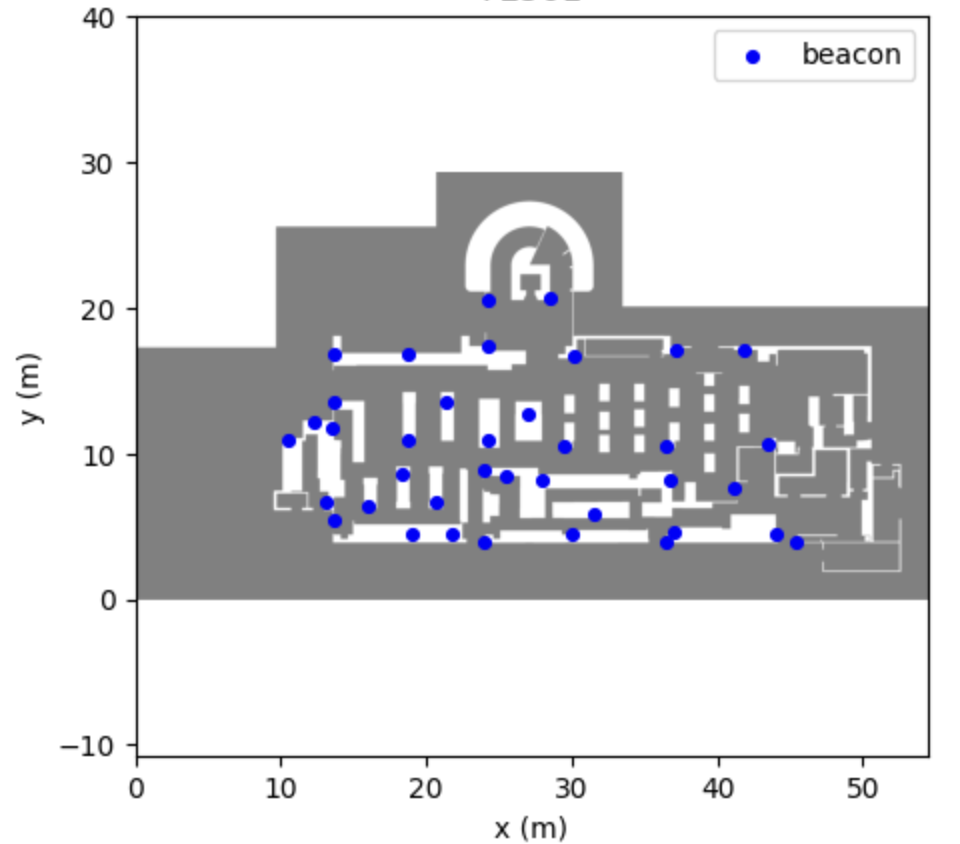
\includegraphics[width=\linewidth]{image/ble-beacon-position.jpg}
	\caption{BLEビーコンの基地局の位置情報}    \label{fig:ble-beacon-position}
\end{figure}

\begin{figure}[ht]
	\centering
	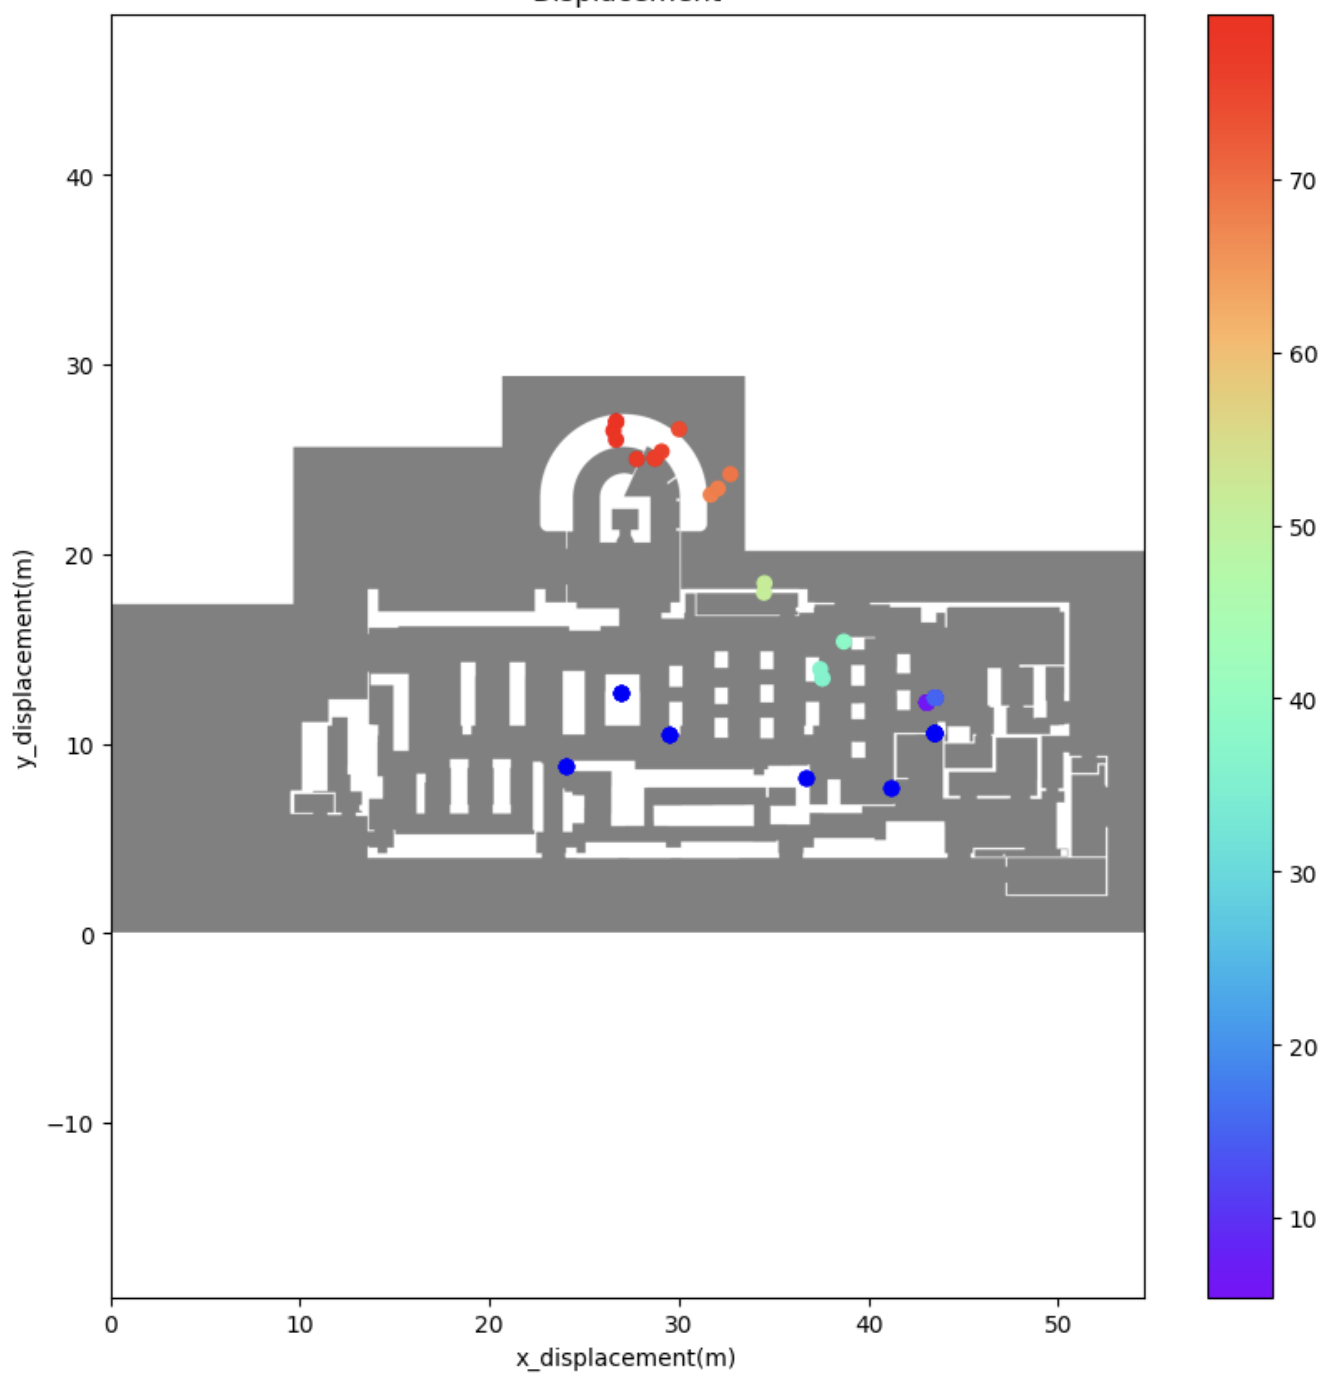
\includegraphics[width=\linewidth]{image/ble-merge.jpg}
	\caption{強いビーコン電波を受信した際の\\時間的に近い軌跡の座標}    \label{fig:ble-merge}
\end{figure}


